\chapter{Introduction to Vectors}

After three chapters of discussion about matrices, it is time to talk about another closely related object type in linear algebra, namely, vectors. While \textit{vectors} and \textit{vector spaces} have strictly mathematical definitions which make them abstract, we will take a more physical point of view with the special case of (finite-dimensional) geometric vectors first.

\section{Definition and Operations of Geometric Vectors}

\subsection{Basic Structure of Vectors in the Real $n$-space $\mathbb{R}^n$}
A \index{Vector}\index{Vector!Geometric Vector}\keywordhl{(geometric) vector} is a physical quantity represented by an ordered tuple of \textit{components} (numbers), e.g. $(1, 8, 7, 4)$, $(1-\imath, 1+3\imath, 2)$. It has a \textit{magnitude (length)} and \textit{direction}, resembling an arrow. Some real-life examples are: two-dimensional flow velocity $(u, v)$, relative position of an airplane to a ground radar $(x, y, z)$.
\begin{defn}[$n$-dimensional Geometric Vector]
\label{defn:geometvec}
A $n$-dimensional geometric vector consists of $n$ ordered elements called \index{Components}\keywordhl{components} and are denoted by either an arrow or boldface, like $\vec{v}$ or $\textbf{v}$. It is usually written out in two forms, as a \textit{column vector} or an \textit{ordered $n$-tuple}:
\begin{align*}
\vec{v} &=
\begin{bmatrix}
v_1 \\
v_2 \\
v_3 \\
\vdots \\
v_n
\end{bmatrix}
=
(v_1, v_2, v_3, \ldots, v_n)^T
\end{align*}
\end{defn}
A $n$-dimensional vector can be treated as an $n \times 1$ (\index{Vector!Column Vector}\keywordhl{column vector}) as suggested above, or a $1 \times n$ matrix (\index{Vector!Row Vector}\keywordhl{row vector}) depending on the situation. The form of a column vector is taken more often than the row vector one and so the column form is assumed throughout the book if it is not further specified. That is why the superscript $^T$ is added for the $n$-tuple form to reflect that it is in fact a column vector despite written horizontally. \par
\begin{tikzpicture}
\draw[->] (-2.5,0)--(2.5,0) node[right]{$x$};
\draw[->] (0,-2.5)--(0,2.5) node[above]{$y$};
\draw[blue,->,line width=1.2] (0,0)--(2,1) node[anchor=south]{$\vec{v} = (2,1)^T$};
\draw[Gray,dashed] (2,1)--(2,0) node[below]{$x = 2$};
\draw[Gray,dashed] (2,1)--(0,1) node[left]{$y = 1$};
\node[below left]{$O$}; 
\end{tikzpicture}\\    
A 2D vector drawn in an x-y plane.\par
{\fbox{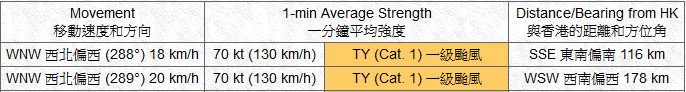
\includegraphics[scale = 0.5]{higos.jpg}}\\
Forecast for \textit{Typhoon Higos} (taken from \href{http://www.hkww.org/weather/tcarchive.html}{Hong Kong Weather Watch}). Its horiztonal movement is a two-dimensional vector, even though the speed and direction are given instead of the velocities in $x$ and $y$-direction (they can be converted to each other).}

Implicit in the definition of $n$-dimensional vectors is the $n$-dimensional \textit{space} they are residing in. Assume the components of those vectors are all real, then the set of all such vectors constitutes the \index{Real $n$-space}\keywordhl{real $n$-space $\mathbb{R}^n$}.
\begin{defn}[The Real $n$-space $\mathbb{R}^n$]
\label{defn:real_nspace}
The real $n$-space $\mathbb{R}^n$ is defined as the set of all possible $n$-tuples $\vec{v} = (v_1, v_2, v_3, \ldots, v_n)^T$ as defined in Definition \ref{defn:geometvec}, where $v_i$ can take any \textit{real} value, for $i = 1,2,3,\ldots,n$. Such objects in $\mathbb{R}^n$ are known as $n$-dimensional \textit{real} vectors.
\end{defn}
While we have not clearly defined what a vector space is, we note that $\mathbb{R}^n$ fulfills the requirements of a vector space in a mathematical sense. A more detailed discussion of this aspect will be deferred to Chapter \ref{chap:vec_space}. Meanwhile, the complex counterpart will be explored in Chapter \ref{chap:complex}.\\
\\
An $n$-dimensional real geometric vectors as described in Definition \ref{defn:geometvec} and \ref{defn:real_nspace} can be written as the sum of $n$ \index{Standard Unit Vector}\keywordhl{standard unit vectors} that have a magnitude of $1$ and are oriented in the positive direction along the $p$-th coordinates axes. They are denoted by $\hat{e}_p$, where $p$ can be from $1$ to $n$. The coordinate axes are perpendicular (or more generally, \textit{orthogonal}, introduced later in this chapter) to each other and this coordinate system is known as the \index{Cartesian Coordinate System}\keywordhl{Cartesian (coordinate) system}. Particularly, in the three-dimensional real space $\mathbb{R}^3$, $\hat{e}_1 = \hat{i} = (1,0,0)^T$, $\hat{e}_2 = \hat{j} = (0,1,0)^T$, $\hat{e}_3 = \hat{k} = (0,0,1)^T$ correspond to "an arrow" of length $1$ pointing in the positive direction of the $x$, $y$, $z$ axes respectively. 
\begin{defn}[Standard Unit Vector]
\label{defn:standardunitvec}
A standard unit vector $\hat{e}_p$ in the real $n$-space $\mathbb{R}^n$ (Definition \ref{defn:real_nspace}) has $n$ components, consisted of $1$ at the $p$-th entry and $0$ elsewhere. Mathematically, for $1\leq q \leq n$, $[\hat{e}_p]_q = 1$ when $q=p$ and $[\hat{e}_p]_q = 0$ when $q\neq p$.
\end{defn}
Below is an example of a geometric vector in the three-dimensional $xyz$ space ($\mathbb{R}^3$).
\begin{center}
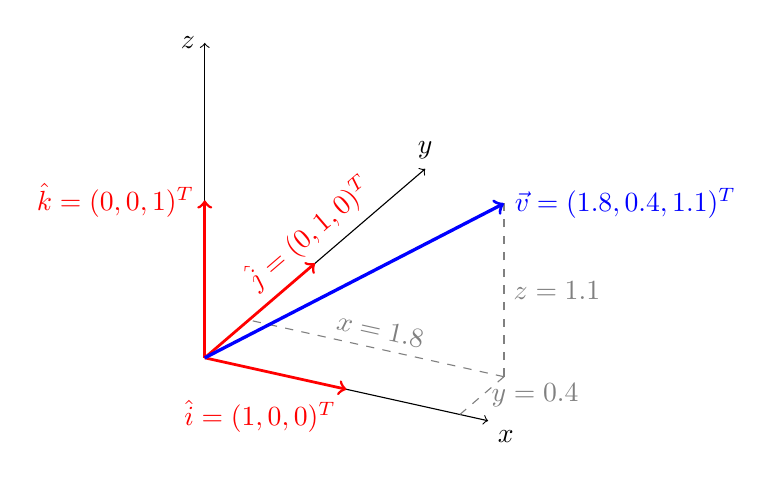
\begin{tikzpicture}[x={(1.8cm, -0.4cm)}, y={(1.4cm, 1.2cm)}, z={(0cm, 2cm)}]
\draw [->] (0,0,0) -- (2,0,0) node [below right] {$x$};
\draw [->] (0,0,0) -- (0,2,0) node [above] {$y$};
\draw [->] (0,0,0) -- (0,0,2) node [left] {$z$};
\draw [->, thick, red, line width=1] (0,0,0) -- (1,0,0) node [below left] {$\hat{i} = (1,0,0)^T$};
\draw [->, thick, red, line width=1] (0,0,0) -- (0,1,0) node [above right, midway, sloped] {$\hat{j} = (0,1,0)^T$} ; 
\draw [->, thick, red, line width=1] (0,0,0) -- (0,0,1) node [left] {$\hat{k} = (0,0,1)^T$};
\draw [Gray, dashed] (1.8,0.4,0) -- (1.8,0,0) node[right, midway]{$y=0.4$}; 
\draw [Gray, dashed] (1.8,0.4,0) -- (0,0.4,0) node[above, midway, sloped]{$x=1.8$}; 
\draw [Gray, dashed] (1.8,0.4,0) -- (1.8,0.4,1.1) node[midway, right]{$z=1.1$};
\draw [->, blue, line width=1.2] (0,0,0) -- (1.8,0.4,1.1) node [right] {$\vec{v} = (1.8,0.4,1.1)^T$};
/\end{tikzpicture}
\begin{align*}
\vec{v} &= 
\begin{bmatrix}
1.8 \\
0.4 \\
1.1
\end{bmatrix}
= 1.8
\begin{bmatrix}
1 \\
0 \\
0
\end{bmatrix}
+ 0.4
\begin{bmatrix}
0 \\
1 \\
0
\end{bmatrix}
+ 1.1
\begin{bmatrix}
0 \\
0 \\
1
\end{bmatrix} 
= 1.8\hat{i} + 0.4\hat{j} + 1.1\hat{k} \\
&= (1.8,0.4,1.1)^T
\end{align*}
\end{center}
where we have written $\vec{v}$ in two forms, as an $n$-tuple and a sum of the three standard unit vectors $\hat{i}, \hat{j}, \hat{k}$.

\subsection{Fundamental Vector Operations}
\label{section:vectoraddmul}
\subsubsection{Addition and Subtraction}
Same as their matrix counterpart, addition and subtraction between vectors are element-wise, and hence only valid for vectors of the same dimension. For $\vec{w} = \vec{u} \pm \vec{v}$, we have $w_i = u_i \pm v_i$. If
\begin{align*}
&\vec{u} =
\begin{bmatrix}
1 \\
2
\end{bmatrix}
&
\vec{v} =
\begin{bmatrix}
2 \\
-1
\end{bmatrix}
\end{align*}
then
\begin{align*}
\vec{u} + \vec{v} =
\begin{bmatrix}
\textcolor{red}{1} \\
\textcolor{red}{2}
\end{bmatrix}
+
\begin{bmatrix}
\textcolor{blue}{2} \\
\textcolor{blue}{-1}
\end{bmatrix}
&= 
\begin{bmatrix}
\textcolor{Green}{3} \\
\textcolor{Green}{1}
\end{bmatrix}
\\
\vec{u} - \vec{v} =
\begin{bmatrix}
\textcolor{red}{1} \\
\textcolor{red}{2}
\end{bmatrix}
-
\begin{bmatrix}
\textcolor{blue}{2} \\
\textcolor{blue}{-1}
\end{bmatrix}
&= 
\begin{bmatrix}
\textcolor{Green}{-1} \\
\textcolor{Green}{3}
\end{bmatrix}
\end{align*}
\begin{center}
\begin{tikzpicture}[scale=0.8]
\draw[->] (-3.5,0)--(3.5,0) node[right]{$x$};
\draw[->] (0,-3.5)--(0,3.5) node[above]{$y$};
\draw[red,-stealth,line width=1] (0,0)--(1,2) node[anchor=south west]{$\vec{u} = (1,2)^T$};
\draw[blue,-stealth,line width=1] (1,2)--(3,1) node[anchor=south west]{$\vec{v} = (2,-1)^T$};
\draw[Green,-stealth,line width=1] (0,0)--(3,1) node[anchor=north west]{$\vec{u} + \vec{v} = (3,1)^T$};
\node[below left]{$O$}; 
\end{tikzpicture}\\
Addition: The tail of the blue vector is placed to the head of the red vector, and the resultant green vector is from the origin to the head of blue vector.
\end{center}
\begin{center}
\begin{tikzpicture}[scale=0.8]
\draw[->] (-3.5,0)--(3.5,0) node[right]{$x$};
\draw[->] (0,-3.5)--(0,3.5) node[above]{$y$};
\draw[red,-stealth,line width=1] (0,0)--(1,2) node[anchor=south west]{$\vec{u} = (1,2)^T$};
\draw[blue,-stealth,line width=1] (1,2)--(-1,3) node[anchor=south east]{$-\vec{v} = (-2,1)^T$};
\draw[Green,-stealth,line width=1] (0,0)--(-1,3) node[anchor=north east]{$\vec{u} - \vec{v} = (-1,3)^T$};
\node[below left]{$O$}; 
\end{tikzpicture}\\
Subtraction: Similar to addition but with the blue vector oriented in the opposite direction.
\end{center}

\subsubsection{Scalar Multiplication} 
Multiplying a scalar (be it a real or complex number) to a vector means that all components are multiplied by that scalar.
\begin{align*}
2
\begin{bmatrix}
2 \\
0 \\
1 \\
9
\end{bmatrix}
=
\begin{bmatrix}
4 \\
0 \\
2 \\
18
\end{bmatrix}
\end{align*}
Looking back at vector subtraction, it can be viewed as addition with a factor of $-1$ in the front.
\begin{align*}
\begin{bmatrix}
7 \\
5 \\
9
\end{bmatrix}
-
\begin{bmatrix}
3 \\
6 \\
9
\end{bmatrix}
=
\begin{bmatrix}
7 \\
5 \\
9
\end{bmatrix}
+ (-1)
\begin{bmatrix}
3 \\
6 \\
9
\end{bmatrix}
=
\begin{bmatrix}
7 \\
5 \\
9
\end{bmatrix}
+
\begin{bmatrix}
-3 \\
-6 \\
-9
\end{bmatrix}
=
\begin{bmatrix}
4 \\
-1 \\
0
\end{bmatrix}
\end{align*}

\subsubsection{Length and Unit Vector} \index{Length}\index{Magnitude}\keywordhl{Length (magnitude)}, or more formally \index{Euclidean Norm}\keywordhl{Euclidean norm}, of a vector $\vec{v}$ is based on a generalized version of \index{Pythagoras’ Theorem}\keywordhl{Pythagoras’ Theorem}, and is evaluated as the square root of the sum of squares of components.
\begin{defn}[Vector Length]
\label{defn:vectorlength}
Length, or magnitude of a $n$-dimensional \textit{real} vector $\vec{v}$, denoted by $\norm{\vec{v}}$, is given by
\begin{align*}
\norm{\vec{v}} &= \sqrt{v_1^2 + v_2^2 + v_3^2 + \cdots + v_n^2} \\
&= \sqrt{\sum_{k=1}^{n} v_k^2}
\end{align*}
\end{defn}
For instance, the length of a two-dimensional vector follows the usual Pythagoras' Theorem as below. \\
\begin{tikzpicture}
\draw[->] (-2.5,0)--(2.5,0) node[right]{$x$};
\draw[->] (0,-2.5)--(0,2.5) node[above]{$y$};
\draw[blue,-stealth,line width=1.2] (0,0)--(2,1) node[anchor=south west, align=left]{$\vec{v} = (2,1)^T$\\$\norm{\vec{v}} = \sqrt{x^2 + y^2} = \sqrt{2^2+1^2} = \sqrt{5}$};
\draw[Gray,dashed] (2,1)--(2,0) node[below]{$x = 2$};
\draw[Gray,dashed] (2,1)--(0,1) node[left]{$y = 1$};
\node[below left]{$O$}; 
\end{tikzpicture}\\
Here is another example which is three-dimensional.
\begin{center}
\begin{tikzpicture}[x={(1.8cm, -0.6cm)}, y={(1.6cm, 1.0cm)}, z={(0cm, 2cm)}]
\draw [->] (-1,0,0) -- (2,0,0) node [right] {$x$};
\draw [->] (0,-1,0) -- (0,2,0) node [above] {$y$};
\draw [->] (0,0,0) -- (0,0,2) node [left] {$z$};
\node[below] (0,0,0){$O$};
\draw [Gray, dashed] (1.6,-0.2,0) -- (1.6,0,0) node[below, pos=-0.5, sloped]{$y=-1$}; 
\draw [Gray, dashed] (1.6,-0.2,0) -- (0,-0.2,0) node[below, midway, sloped]{$x=8$}; 
\draw [Gray, dashed] (1.6,-0.2,0) -- (1.6,-0.2,0.8) node[midway, right]{$z=4$};
\draw [->, blue, line width=1.2] (0,0,0) -- (1.6,-0.2,0.8) node [right] {$\vec{w} = (8,-1,4)^T$};
\end{tikzpicture}
\begin{align*}
\vec{w} &= 
\begin{bmatrix}
8 \\
-1 \\
4
\end{bmatrix}
& \norm{\vec{w}}&=
\sqrt{8^2 + (-1)^2 + 4^2} = 9 
\end{align*}
\end{center}
We can create a \index{Vector!Unit Vector}\keywordhl{unit vector} that has a length of $1$ from any vector $\vec{v}$ and orients in the same direction as $\vec{v}$. It is simply created by dividing (normalizing) $\vec{v}$ by its distance $\norm{\vec{v}}$.
\begin{defn}[Unit Vector]
\label{defn:unitvec}
The unit vector corresponding to a non-zero vector $\vec{v}$ is denoted as $\hat{v}$ and is given by
\begin{align*}
\hat{v} &= \frac{1}{\norm{\vec{v}}}\vec{v}
\end{align*}
where the length $\norm{\vec{v}}$ is defined as in Definition \ref{defn:vectorlength}. 
\end{defn}
Note that despite vectors can carry physical units, unit vectors are all physically \textit{dimensionless} when formulated in this way. \\
\\
Short Exercise: Find the unit vector for $\vec{w} = (8, -1, 4)^T$ in the previous example, and verify that it has a length of $1$.\footnote{$\norm{\vec{w}} = 9$, $\hat{w} = \frac{\vec{w}}{\norm{\vec{w}}} = \frac{1}{9}(8,-1,4)^T = (\frac{8}{9}, -\frac{1}{9}, \frac{4}{9})^T$, $\norm{\hat{w}} = \sqrt{(\frac{8}{9})^2 + (-\frac{1}{9})^2 + (\frac{4}{9})^2} = 1$.}

\section{Special Vector Operations}
\label{section:vectorops}
Now we are going to introduce two special types of vector operations: \textit{dot product}, and \textit{cross product}. 

\subsection{Dot Product}
\index{Dot Product}\keywordhl{(Real) Dot product} (or \index{Scalar Product}\keywordhl{scalar product}) is defined for two (real) vectors that have the same number of dimension. It is the sum of products of paired components between the two vectors. In other words, it can be regarded to be the matrix product between a row vector ($1 \times m$ matrix) and a column vector ($m \times 1$ matrix). 
\begin{defn}[Dot Product (Real)]
\label{defn:dotreal}
The dot product between two $n$-dimensional \textit{real} vectors $\vec{u}$ and $\vec{v}$ in $\mathbb{R}^n$ are denoted as either $\vec{u} \cdot \vec{v}$, or by matrix notation $\textbf{u}^T\textbf{v}$. They are defined as
\begin{align*}
\vec{u} \cdot \vec{v} = \textbf{u}^T\textbf{v} &= u_1v_1 + u_2v_2 + u_3v_3 + \cdots + u_nv_n \\
&= \sum_{k=1}^{n} u_kv_k
\end{align*}
which is a scalar quantity.
\end{defn}
Conversely, it can be said that entries of a matrix product are vector dot products between the corresponding rows and columns. It is emphasized that we are restricting ourselves to real entries since complex vectors introduce a bit of extra complications. Then, for two \textit{real} matrices expressed in the form of combined row/column vectors that are $\mathbb{R}^n$,
\begin{align*}
A &= \left[\begin{array}{@{}c@{}}
\text{---} \vec{u}^{(1)T} \text{---} \\
\hline
\text{---} \vec{u}^{(2)T} \text{---} \\
\hline
\vdots \\
\hline
\text{---} \vec{u}^{(p)T} \text{---}
\end{array}\right]
=  \left[\begin{array}{@{}c|c|c|c@{}}
| & | & & | \\
\vec{u}^{(1)} & \vec{u}^{(2)} & \cdots & \vec{u}^{(p)} \\
| & | & & |
\end{array}\right]^T
& B &= \left[\begin{array}{@{}c|c|c|c@{}}
| & | & & | \\
\vec{v}^{(1)} & \vec{v}^{(2)} & \cdots & \vec{v}^{(q)} \\
| & | & & |
\end{array}\right]\\
&= 
\begin{bmatrix}
\vec{u}^{(1)}_1  & \vec{u}^{(1)}_2 & \cdots & \vec{u}^{(1)}_n \\
\vec{u}^{(2)}_1  & \vec{u}^{(2)}_2 & \cdots & \vec{u}^{(2)}_n \\
\vdots & \vdots & & \vdots \\
\vec{u}^{(p)}_1  & \vec{u}^{(p)}_2 & \cdots & \vec{u}^{(p)}_n
\end{bmatrix} 
& &= 
\begin{bmatrix}
\vec{v}^{(1)}_1  & \vec{v}^{(2)}_1 & \cdots & \vec{v}^{(q)}_1 \\
\vec{v}^{(1)}_2  & \vec{v}^{(2)}_2 & & \vec{v}^{(q)}_2 \\
\vdots & & \ddots & \vdots \\
\vec{v}^{(1)}_n  & \vec{v}^{(2)}_n & \cdots & \vec{v}^{(q)}_n \\
\end{bmatrix} 
\end{align*}
(notice those transposes in the expression of $A$) their matrix product $AB$ can be written as
\begin{align*}
AB =
\begin{bmatrix}
\vec{u}^{(1)} \cdot \vec{v}^{(1)} & \vec{u}^{(1)} \cdot \vec{v}^{(2)} & \cdots & \vec{u}^{(1)} \cdot \vec{v}^{(q)} \\
\vec{u}^{(2)} \cdot \vec{v}^{(1)} & \vec{u}^{(2)} \cdot \vec{v}^{(2)} & \cdots & \vec{u}^{(2)} \cdot \vec{v}^{(q)} \\
\vdots & \vdots & & \vdots \\
\vec{u}^{(p)} \cdot \vec{v}^{(1)} & \vec{u}^{(p)} \cdot \vec{v}^{(2)} & \cdots & \vec{u}^{(p)} \cdot \vec{v}^{(q)} \\
\end{bmatrix}
\end{align*}
We can use dot product to express the length of a real vector.
\begin{proper}
\label{proper:lengthdot}
The length of a real vector, as defined in Definition \ref{defn:vectorlength}, can be written using its dot product between itself as
\begin{align*}
\norm{\vec{v}} &= \sqrt{\vec{v} \cdot \vec{v}} & &\text{or} &
\norm{\vec{v}}^2 &= \vec{v} \cdot \vec{v}
\end{align*}
\end{proper}
Notice that $\vec{v} \cdot \vec{v} = v_1^2 + v_2^2 + v_3^2 + \cdots + v_n^2 \geq 0$. This quantity is always strictly greater than zero ($\vec{v} \cdot \vec{v} > 0$) unless $\vec{v} = \textbf{0}$ is the zero vector (then $\vec{v} \cdot \vec{v} = 0$), which makes sense physically given that it represents length.

\begin{exmp}
\label{exmp:dotproduct5d}
If $\vec{u} = (1, 2, 3, 4, 5)^T$ and $\vec{v} = (-1, 0, 2, 1, -2)^T$, find the dot product $\vec{u} \cdot \vec{v} = \textbf{u}^T\textbf{v}$.
\end{exmp}
\begin{solution}
\begin{align*}
\vec{u} \cdot \vec{v} &= (1)(-1) + (2)(0) + (3)(2) + (4)(1) + (5)(-2) = -1
\end{align*}
Alternatively,
\begin{align*}
\textbf{u}^T\textbf{v} &=
\begin{bmatrix}
1 & 2 & 3 & 4 & 5
\end{bmatrix}
\begin{bmatrix}
-1 \\
0 \\
2 \\
1 \\
-2
\end{bmatrix}
= -1
\end{align*}
\end{solution}

Here are some properties of dot product.
\begin{proper}
\label{proper:dotproper}
For three $n$-dimensional real vectors $\vec{u}$, $\vec{v}$ and $\vec{w}$, the following properties hold.
\begin{align*}
\vec{u} \cdot \vec{v} &= \vec{v} \cdot \vec{u} &\text{Symmetry Property} \\
\vec{u} \cdot (\vec{v} \pm \vec{w}) &= \vec{u} \cdot \vec{v} \pm \vec{u} \cdot \vec{w} &\text{Distributive Property} \\
(\vec{u} \pm \vec{v}) \cdot \vec{w} &= \vec{u} \cdot \vec{w} \pm \vec{v} \cdot \vec{w} &\text{Distributive Property} \\
(a\vec{u}) \cdot (b\vec{v}) &= ab(\vec{u} \cdot \vec{v}) &\text{where $a$, $b$ are some constants}
\end{align*}
Additionally, if $A$ is an $n \times n$ square matrix, then
\begin{align*}
\vec{u} \cdot (A\vec{v}) &= \textbf{u}^T(A\textbf{v}) = (A^T\textbf{u})^T\textbf{v} = (A^T\vec{u}) \cdot \vec{v} \\
(A\vec{u}) \cdot \vec{v} &= (A\textbf{u})^T\textbf{v} = \textbf{u}^T(A^T\textbf{v}) = \vec{u} \cdot (A^T\vec{v})
\end{align*}
where we have used Definition \ref{defn:dotreal} and Properties \ref{proper:transp}.
\end{proper}
\begin{exmp}
For $\vec{u} = (1,3,1)^T$ and $\vec{v} = (2,-1,1)^T$, find $\norm{(\vec{u} + \vec{v})}^2 = (\vec{u} + \vec{v}) \cdot (\vec{u} + \vec{v})$.
\end{exmp}
\begin{solution}
By Properties \ref{proper:dotproper}, we can rewrite the expression as
\begin{align*}
(\vec{u} + \vec{v}) \cdot (\vec{u} + \vec{v}) &= \vec{u} \cdot (\vec{u} + \vec{v}) + \vec{v} \cdot (\vec{u} + \vec{v}) \\
&= \vec{u} \cdot \vec{u} + \vec{u} \cdot \vec{v} + \vec{v} \cdot \vec{u} + \vec{v} \cdot \vec{v} \\
&= \vec{u} \cdot \vec{u} + 2 \vec{u} \cdot \vec{v} + \vec{v} \cdot \vec{v}
\end{align*}
Subsequently,
\begin{align*}
&\quad \vec{u} \cdot \vec{u} + 2 \vec{u} \cdot \vec{v} + \vec{v} \cdot \vec{v} \\
&= (1,3,1)^T \cdot (1,3,1)^T + 2((1,3,1)^T \cdot (2,-1,1)^T) + (2,-1,1)^T \cdot (2,-1,1)^T \\
&= (1^2 + 3^2 + 1^2) + 2((1)(2)+(3)(-1)+(1)(1)) + (2^2 + (-1)^2 + 1^2) \\
&= 11 + 2(0) + 6 \\
&= 17
\end{align*}
Alternatively, one can calculate $\vec{w} = \vec{u} + \vec{v} = (1,3,1)^T + (2,-1,1)^T = (3,2,2)^T$ and find $\vec{w} \cdot \vec{w} = \norm{\vec{w}}^2$ instead. (which is easier and faster)
\end{solution}
\begin{exmp}
Given $\vec{u}$ and $\vec{v}$ as defined in the example above, if
\begin{align*}
A =
\begin{bmatrix}
1 & 2 & 1 \\
2 & 0 & 3 \\
1 & 1 & -1
\end{bmatrix}
\end{align*}
verify that $\vec{u} \cdot (A\vec{v}) = (A^T\vec{u}) \cdot \vec{v}$.
\end{exmp}
\begin{solution}
\begin{align*}
A\vec{v} &= 
\begin{bmatrix}
1 & 2 & 1 \\
2 & 0 & 3 \\
1 & 1 & -1
\end{bmatrix}
\begin{bmatrix}
2 \\
-1 \\
1
\end{bmatrix} \\
&=
\begin{bmatrix}
(1)(2) + (2)(-1) + (1)(1) \\
(2)(2) + (0)(-1) + (3)(1) \\
(1)(2) + (1)(-1) + (-1)(1) 
\end{bmatrix} \\
&=
\begin{bmatrix}
1 \\
7 \\
0
\end{bmatrix} \\
\vec{u} \cdot (A\vec{v}) &= (1,3,1)^T \cdot (1,7,0)^T \\
&= (1)(1) + (3)(7) + (1)(0) \\
&= 22
\end{align*}
On the other hand,
\begin{align*}
A^T\vec{u} &= 
\begin{bmatrix}
1 & 2 & 1 \\
2 & 0 & 1 \\
1 & 3 & -1
\end{bmatrix}
\begin{bmatrix}
1 \\
3 \\
1
\end{bmatrix} \\
&=
\begin{bmatrix}
(1)(1) + (2)(3) + (1)(1) \\
(2)(1) + (0)(3) + (1)(1) \\
(1)(1) + (3)(3) + (-1)(1) 
\end{bmatrix} \\
&=
\begin{bmatrix}
8 \\
3 \\
9
\end{bmatrix} \\
(A^T\vec{u}) \cdot \vec{v} &= (8,3,9)^T \cdot (2,-1,1)^T \\
&= (8)(2) + (3)(-1) + (9)(1) \\
&= 22
\end{align*}
\end{solution}

\subsubsection{Geometric Meaning of Dot Product}
The geometric meaning of dot product is embedded in the relation below.
\begin{proper}
\label{proper:dotgeo}
For two real vectors $\vec{u}$ and $\vec{v}$ that are of the same dimension, we have
\begin{align*}
\vec{u} \cdot \vec{v} = \norm{\vec{u}}\norm{\vec{v}}\cos\theta
\end{align*}
where $\theta$ is the angle between $\vec{u}$ and $\vec{v}$. Furthermore, if $\hat{u}$ and $\hat{v}$ are unit vectors (Definition \ref{defn:unitvec}) such that $\norm{\vec{u}} = \norm{\vec{v}} = 1$, it reduces to
\begin{align*}
\hat{u} \cdot \hat{v} = \cos\theta    
\end{align*}
\end{proper}
This means that the dot product between two vectors $\vec{u}$ and $\vec{v}$ is geometrically the signed product between $\vec{u}$ and the parallel component (projection) of $\vec{v}$ onto $\vec{u}$ (or vice versa), which is illustrated in the figure below. While an angle has a clear physical meaning only in a two/three-dimensional space, such relation generalizes the idea of an angle to higher dimensions.
\begin{center}
\begin{tikzpicture}[scale=1.3]
\coordinate (0) at (0,0);
\coordinate (vecu) at (4,1);
\coordinate (vecv) at (1,2);
\draw[->](0)--(vecu) node[right]{$\vec{u}$};
\draw[->](0)--(vecv) node[above]{$\vec{v}$};
\draw[dashed] (1,2)--(24/17, 6/17);
\draw[red] (24/17+0.2, 6/17+0.05)--(24/17+0.15, 6/17+0.25)--(24/17-0.05, 6/17+0.2);
\pic[draw, "$\theta$", angle eccentricity=1.5] {angle = vecu--0--vecv};
\draw[blue, very thick] (0,0)--(24/17, 6/17) node[below, shift={(0mm, -2mm)}]{$\norm{\vec{v}}\cos\theta$};
\end{tikzpicture}
\end{center}
\begin{exmp}
Find the angle between $\vec{u}$ and $\vec{v}$ in Example \ref{exmp:dotproduct5d}.
\end{exmp}
\begin{solution}
From Example \ref{exmp:dotproduct5d}, we have $\vec{u} \cdot \vec{v} = -1$, and
\begin{align*}
\norm{\vec{u}} &= \sqrt{1^2 + 2^2 + 3^2 + 4^2 + 5^2} = \sqrt{55} \\
\norm{\vec{v}} &= \sqrt{(-1)^2 + 0^2 + 2^2 + 1^2 + (-2)^2} = \sqrt{10} 
\end{align*}
By Properties \ref{proper:dotgeo}, we have
\begin{align*}
\cos\theta &= \frac{\vec{u} \cdot \vec{v}}{\norm{\vec{u}}\norm{\vec{v}}} \\
&= \frac{-1}{(\sqrt{55})(\sqrt{10})} \\
&\approx -0.0426 \\
\theta &\approx \SI{1.613}{\radian} = \SI{92.44}{\degree}
\end{align*}
\end{solution}
By Properties \ref{proper:dotgeo}, if the absolute value of the dot product $|\vec{u} \cdot \vec{v}|$ is equal to $\norm{\vec{u}}\norm{\vec{v}}$, where $\vec{u}$ and $\vec{v}$ are non-zero vectors, then it implies that $\cos\theta = \pm 1$, $\theta$ is either $0$ or $\pi$, and hence the two vectors are parallel. In constrast,
\begin{proper}
\label{proper:dotorth}
If the dot product between two real vectors $\vec{u}$ and $\vec{v}$ is zero ($\vec{u} \cdot \vec{v} = \vec{v} \cdot \vec{u} = 0$), then by Properties \ref{proper:dotgeo}, $\cos\theta = 0$ and the angle $\theta$ between $\vec{u}$ and $\vec{v}$ is $\frac{\pi}{2}$. In this case, $\vec{u}$ and $\vec{v}$ are said to be perpendicular, or \textit{orthogonal} to each other.
\end{proper}
From this, the concept of "\index{Orthogonal}\keywordhl{orthogonal}" becomes an extension of "perpendicular" in higher dimensions. It is easy to see that the standard unit vectors of $\mathbb{R}^n$ are orthogonal. Note that \textit{the zero vector is regarded to be orthogonal to any vector}, so even if $\vec{u}$ or $\vec{v}$ is a zero vector, this properties still hold. \par
Some may notice that as $-1 \leq \cos\theta \leq 1$, if $|\vec{u} \cdot \vec{v}| > \norm{\vec{u}}\norm{\vec{v}}$, then $\theta$ in Properties \ref{proper:dotgeo} will be ill-defined. However, the \index{Cauchy–Schwarz Inequality}\keywordhl{Cauchy–Schwarz Inequality} ensures this will not happen.
\begin{thm}[Cauchy–Schwarz Inequality]
\label{thm:CauchySch}
Given two \textit{real} $n$-dimensional vectors $\vec{u}$ and $\vec{v}$ ($\vec{u}, \vec{v} \in \mathbb{R}^n$), the following inequality holds.
\begin{align*}
|\vec{u} \cdot \vec{v}| &\leq \norm{\vec{u}}\norm{\vec{v}} \\
|u_1v_1+u_2v_2+\cdots+u_nv_n| &\leq \sqrt{u_1^2+u_2^2+\cdots+u_n^2}\sqrt{v_1^2+v_2^2+\cdots+v_n^2}
\end{align*}
\end{thm}
\begin{proof}
Consider $\vec{w} = \vec{u} + t\vec{v}$, where $t$ is any scalar, then $\norm{\vec{w}}^2 = \vec{w}\cdot\vec{w} \geq 0$ by Properties \ref{proper:lengthdot}. Also, $\vec{w}\cdot\vec{w}$ can be written as a quadratic polynomial in $t$:
\begin{align*}
\vec{w}\cdot\vec{w} = (\vec{u} + t\vec{v}) \cdot (\vec{u} + t\vec{v}) = \norm{\vec{u}}^2 + 2t(\vec{u} \cdot \vec{v}) + t^2\norm{\vec{v}}^2
\end{align*}
Since this quantity is always greater than or equal to zero, i.e.\ the quadratic polynomial has no root or a repeated root, it means that the discriminant must be negative or zero. So,
\begin{align*}
\Delta = b^2 - 4ac &\leq 0 \\
(2(\vec{u} \cdot \vec{v}))^2 - 4\norm{\vec{u}}^2\norm{\vec{v}}^2 &\leq 0 \\
(\vec{u} \cdot \vec{v})^2 - \norm{\vec{u}}^2\norm{\vec{v}}^2 &\leq 0 \\
(\vec{u} \cdot \vec{v})^2 &\leq \norm{\vec{u}}^2\norm{\vec{v}}^2 \\
|\vec{u} \cdot \vec{v}| &\leq \norm{\vec{u}}\norm{\vec{v}}
\end{align*}
\end{proof}
Short Exercise: Think about under what circumstances the Cauchy–Schwarz Inequality turns into an equality (i.e.\ $|\vec{u} \cdot \vec{v}| = \norm{\vec{u}}\norm{\vec{v}}$).\footnote{When $\vec{u}$ and $\vec{v}$ are parallel, i.e. $\vec{u} = k\vec{v}$ for some scalar $k$, or $\vec{v} = \textbf{0}$.}

\begin{exmp}
Prove the \index{Cosine Law}\keywordhl{Cosine Law} by considering the triangle below
\begin{center}
\begin{tikzpicture}
\coordinate (0) at (0,0);
\draw[red,-{Latex[length=5mm, width=2mm]}] (0)--(5,1) node[right](vecu){$\vec{u}$};
\draw[blue,-{Latex[length=5mm, width=2mm]}] (0)--(-1,3) node[above](vecv){$\vec{v}$};
\pic[draw, "$\theta$", angle eccentricity=1.5] {angle = vecu--0--vecv};
\draw[Green,-{Latex[length=5mm, width=2mm]}] (-1,3)--(5,1) node[midway, above, shift={(0mm, 3mm)}]{$\vec{u} - \vec{v}$};
\end{tikzpicture}
\end{center}
and expanding the dot product $\norm{(\vec{u}-\vec{v})}^2 = (\vec{u}-\vec{v}) \cdot (\vec{u}-\vec{v})$.    
\end{exmp}
\begin{solution}
Let denote the lengths $\norm{\vec{u}}$, $\norm{\vec{v}}$, $\norm{(\vec{u}-\vec{v})}$ be $a$, $b$, $c$, then
\begin{align*}
c^2 = \norm{(\vec{u}-\vec{v})}^2 &= (\vec{u}-\vec{v}) \cdot (\vec{u}-\vec{v}) & \text{(Properties \ref{proper:lengthdot})} \\
&= \vec{u} \cdot \vec{u} - \vec{u} \cdot \vec{v} - \vec{v} \cdot \vec{u} + \vec{v} \cdot \vec{v} & \text{(Properties \ref{proper:dotproper})} \\
&= \norm{\vec{u}}^2 - 2\vec{u} \cdot \vec{v} + \norm{\vec{v}}^2 & \text{(Properties \ref{proper:lengthdot} and \ref{proper:dotproper})} \\
&= \norm{\vec{u}}^2 - 2\norm{\vec{u}}\norm{\vec{v}}\cos\theta + \norm{\vec{v}}^2 & \text{(Properties \ref{proper:dotgeo})} \\
&= a^2 - 2ab\cos\theta + b^2
\end{align*}
\end{solution}

\subsection{Cross Product}
\label{section:crossprod}
Another important type of vector product is the \index{Cross Product}\keywordhl{cross product} (or sometimes just \index{Vector Product}\keywordhl{vector product}), which produces a three-dimensional real vector from two other three-dimensional real vectors. \textit{The output vector will be orthogonal to the two input vectors}, and the direction is determined by the \index{Right Hand Rule}\keywordhl{right hand rule}. Motivated by these requirements, we have the following basic definitions of cross product between the three standard unit vectors in $\mathbb{R}^3$.
\begin{defn}
\label{defn:crossijk}
The computation of cross products (denoted by $\times$) involving any two of the standard unit vectors $\hat{i}$, $\hat{j}$, $\hat{k}$ in $\mathbb{R}^3$ obeys the following rules.
\begin{enumerate}
\item $\hat{i} \times \hat{j} = \hat{k}$, $\hat{j} \times \hat{i} = -\hat{k}$,
\item $\hat{j} \times \hat{k} = \hat{i}$, $\hat{k} \times \hat{j} = -\hat{i}$,
\item $\hat{k} \times \hat{i} = \hat{j}$, $\hat{i} \times \hat{k} = -\hat{j}$, and
\item $\hat{i} \times \hat{i} = \hat{j} \times \hat{j} = \hat{k} \times \hat{k} = \textbf{0}$
\end{enumerate}
\end{defn}
\begin{minipage}{0.45\textwidth}
\begin{center}
% https://tex.stackexchange.com/questions/287284/drawing-a-diagram-of-a-three-cycle
\begin{tikzpicture}[->,scale=2]
   \node (i) at (90:1cm)  {\huge$\hat{i}$};
   \node (j) at (-30:1cm) {\huge$\hat{j}$};
   \node (k) at (210:1cm) {\huge$\hat{k}$};

   \draw (70:1cm)  arc (70:-10:1cm);
   \draw (-50:1cm) arc (-50:-130:1cm);
   \draw (190:1cm) arc (190:110:1cm);
\end{tikzpicture} \\
\end{center}
A cyclic diagram for memorizing Definition \ref{defn:crossijk}. A clockwise / anti-clockwise permutation produces a positive / negative unit vector of the third.
\end{minipage}
\hfill
\begin{minipage}{0.5\textwidth}
\begin{center}
% https://tikz.net/righthand_rule/
\begin{tikzpicture}[scale=0.8]
  \coordinate (O) at (1.0,0.7);
  \coordinate (WT) at ( 2.9,-1.1);
  \coordinate (T1) at ( 2.3, 0.7);
  \coordinate (T2) at ( 1.75, 2.3);
  \coordinate (T3) at ( 2.0, 3.1);
  \coordinate (T4) at (1.38, 3.15);
  \coordinate (T5) at ( 0.9, 2.3);
  \coordinate (T6) at ( 0.85, 1.2);
  \coordinate (T7) at ( 0.85, 0.2);
  \coordinate (I1) at (-1.1, 2.45);
  \coordinate (I2) at (-2.9, 3.45);
  \coordinate (I3) at (-3.3, 2.9);
  \coordinate (I4) at (-1.5, 1.8);
  \coordinate (I5) at (-0.9, 1.1);
  \coordinate (I6) at (-0.9, 0.3);
  \coordinate (M1) at (-2.1, 0.9);
  \coordinate (M2) at (-3.95,0.55);
  \coordinate (M3) at (-4.0,-0.15);
  \coordinate (M4) at (-2.3, 0.05);
  \coordinate (M5) at (-1.1, 0.20);
  \coordinate (R1) at (-1.9,-0.1);
  \coordinate (R2) at (-1.8,-0.7);
  \coordinate (R3) at (-0.3,-1.5);
  \coordinate (R4) at ( 0.1,-1.7);
  \coordinate (R5) at ( 0.1,-1.0);
  \coordinate (R6) at (-0.5,-0.7);
  \coordinate (R7) at (-1.2,-0.3);
  \coordinate (P1) at (-1.9,-1.3);
  \coordinate (P2) at (-0.8,-1.9);
  \coordinate (P3) at (-0.2,-2.1);
  \coordinate (P4) at (-0.05,-1.65);
  \coordinate (W1) at ( 0.4,-2.9);
  \coordinate (W2) at ( 1.6,-3.5);
  
  % HAND
  \fill[pink!25]
    (WT) -- (T6) -- (I5) -- (M5) -- (R2) -- (P2) -- (W2) to[out=25,in=-90] cycle;
  \draw[fill=pink!25]
    (WT) to[out=120,in=-60]
    (T1) to[out=120,in=-90]
    (T2) to[out=80,in=-110]
    (T3) to[out=80,in=50,looseness=1.5]
    (T4) to[out=-130,in=80]
    (T5) to[out=-100,in=70]
    (T6) to[out=-100,in=100]
    (T7)
    (T6) to[out=150,in=-30]
    (I1) to[out=150,in=-30]
    (I2) to[out=150,in=145,looseness=1.7]
    (I3) to[out=-30,in=150]
    (I4) to[out=-30,in=105]
    (I5) to[out=-75,in=90]
    (I6)
    (I5) to[out=-170,in=10]
    (M1) to[out=-170,in=10]
    (M2) to[out=-170,in=-175,looseness=1.8]
    (M3) to[out=5,in=-170]
    (M4) to[out=10,in=-170]
    (M5)
    (M5) to[out=-160,in=50]
    (R1) to[out=-130,in=140,looseness=1.2]
    (R2) to[out=-30,in=160]
    (R3) --
    (R4) to[out=-20,in=-20,looseness=1.5]
    (R5) --
    (R6) to[out=140,in=8,looseness=0.9]
    (R7)
    (R2) to[out=-160,in=155]
    (P1) to[out=-35,in=150]
    (P2) to[out=-30,in=160]
    (P3) to[out=-20,in=-30,looseness=1.5]
    (R4)
    (P2) to[out=-50,in=140]
    (W1) to[out=-40,in=160]
    (W2);
    
  \draw[->, blue, line width=1] (O) -- (128:3.2) coordinate(X) node[above=6,left=-6,scale=1.5] {$\vec{u}$};
  \draw[->, red, line width=1] (O) -- (-182:3.2) coordinate(Y) node[above=5,left=-6,scale=1.5] {$\vec{v}$};
  \draw[->, Purple, line width=2] (O) -- (62:3.2) node[above=-1,scale=1.5] {$\textcolor{blue}{\vec{u}} \textcolor{Purple}{\;\times\;} \textcolor{red}{\vec{v}}$};
  \draw pic[->, "$\theta$", draw=black, thick, angle radius=30, angle eccentricity=1.2] {angle = X--O--Y};
\end{tikzpicture}\\
Demonstration of the right hand rule.
\end{center}
\end{minipage}
\par
The properties of cross product are noted below. One major difference setting cross product apart from the dot product is its anti-symmetric property.
\begin{proper}
\label{proper:crossproper}
For two $\mathbb{R}^3$ vectors $\vec{u}$ and $\vec{v}$, we have
\begin{align*}
\vec{u} \times \vec{v} &= -\vec{v} \times \vec{u} &\text{Anti-symmetry Property} \\
\vec{u} \times (\vec{v} \pm \vec{w}) &= \vec{u} \times \vec{v} \pm \vec{u} \times \vec{w} &\text{Distributive Property} \\
(\vec{u} \pm \vec{v}) \times \vec{w} &= \vec{u} \times \vec{w} \pm \vec{v} \times \vec{w} &\text{Distributive Property} \\
(a\vec{u}) \times (b\vec{v}) &= ab(\vec{u} \times \vec{v}) &\text{where $a$, $b$ are some constants}
\end{align*}
\end{proper}
The calculation of cross product then follows from these rules, leading to the determinant shorthand below. 
\begin{proper}
\label{proper:crossdet}
For $\vec{u} = (u_1, u_2, u_3)^T, \vec{v} = (v_1, v_2, v_3)^T \in \mathbb{R}^3$, their cross product $\vec{u} \times \vec{v}$ can be written in the form of a determinant as
\begin{align*}
\vec{u} \times \vec{v} =
\begin{vmatrix}
\hat{i} & \hat{j} & \hat{k} \\
u_1 & u_2 & u_3 \\
v_1 & v_2 & v_3
\end{vmatrix}
\end{align*}
\end{proper}
\begin{proof}
Starting from Definition \ref{defn:crossijk} and Properties \ref{proper:crossproper}, we have
\begin{align*}
\vec{u} \times \vec{v} &= (u_1\hat{i} + u_2\hat{j} + u_3\hat{k}) \times (v_1\hat{i} + v_2\hat{j} + v_3\hat{k}) \\
&= u_1v_1(\hat{i}\times\hat{i}) + u_1v_2(\hat{i}\times\hat{j}) + u_1v_3(\hat{i}\times\hat{k}) \\
&\quad +u_2v_1(\hat{j}\times\hat{i}) + u_2v_2(\hat{j}\times\hat{j}) + u_2v_3(\hat{j}\times\hat{k}) \\
&\quad +u_3v_1(\hat{k}\times\hat{i}) + u_3v_2(\hat{k}\times\hat{j}) + u_3v_3(\hat{k}\times\hat{k}) & \text{(Properties \ref{proper:crossproper})}\\
&= u_1v_1(\textbf{0}) + u_1v_2(\hat{k}) - u_1v_3(\hat{j}) \\
&\quad -u_2v_1(\hat{k}) + u_2v_2(\textbf{0}) + u_2v_3(\hat{i}) \\
&\quad +u_3v_1(\hat{j}) - u_3v_2(\hat{i}) + u_3v_3(\textbf{0}) & \text{(Definition \ref{defn:crossijk})}\\
&= (u_2v_3 - u_3v_2)\hat{i} + (u_3v_1 - u_1v_3)\hat{j} + (u_1v_2 - u_2v_1)\hat{k} 
\end{align*}
Meanwhile, cofactor expansion (Properties \ref{proper:cofactorex}) along the first row of the given determinant form
\begin{align*}
\begin{vmatrix}
\hat{i} & \hat{j} & \hat{k} \\
u_1 & u_2 & u_3 \\
v_1 & v_2 & v_3
\end{vmatrix} 
&= 
\hat{i}
\begin{vmatrix}
u_2 & u_3 \\
v_2 & v_3
\end{vmatrix} 
- \hat{j}
\begin{vmatrix}
u_1 & u_3 \\
v_1 & v_3
\end{vmatrix} 
+ \hat{k}
\begin{vmatrix}
u_1 & u_2 \\
v_1 & v_2
\end{vmatrix} \\
&= (u_2v_3 - u_3v_2)\hat{i} + (u_3v_1 - u_1v_3)\hat{j} + (u_1v_2 - u_2v_1)\hat{k}
\end{align*}
yields the identical result.
\end{proof}

\begin{exmp}
Given two $\mathbb{R}^3$ vectors
\begin{align*}
&\vec{u} =
\begin{bmatrix}
1 \\
0 \\
2
\end{bmatrix}
&\vec{v} =
\begin{bmatrix}
3 \\
-1 \\
1
\end{bmatrix}
\end{align*}
Find $\vec{u} \times \vec{v}$.
\end{exmp}
\begin{solution}
\begin{align*}
\vec{u} \times \vec{v} &=
\begin{vmatrix}
\hat{i} & \hat{j} & \hat{k} \\
1 & 0 & 2 \\
3 & -1 & 1
\end{vmatrix} \\
&= 
\hat{i}
\begin{vmatrix}
0 & 2 \\
-1 & 1 
\end{vmatrix}
- \hat{j}
\begin{vmatrix}
1 & 2 \\
3 & 1 
\end{vmatrix}
+ \hat{k}
\begin{vmatrix}
1 & 0 \\
3 & -1 
\end{vmatrix}
& \begin{aligned}
\text{(Cofactor expansion} \\ 
\text{along the first row)}
\end{aligned}\\
&= 2\hat{i} + 5\hat{j} - \hat{k} = (2,5,-1)^T
\end{align*} 
\end{solution}
Short Exercise: Check if $\vec{u} \times \vec{v}$ is orthogonal to $\vec{u}$ and $\vec{v}$ by finding the corresponding dot products.\footnote{$\vec{u} \cdot (\vec{u} \times \vec{v}) = (1,0,2)^T\cdot(2,5,-1)^T = (1)(2) + (0)(5) + (2)(-1) = 0$, $\vec{v} \cdot (\vec{u} \times \vec{v}) = (3,-1,1)^T\cdot(2,5,-1)^T = (3)(2) + (-1)(5) + (1)(-1) = 0$. The zero dot product in both cases  shows they are orthogonal via Properties \ref{proper:dotorth}.}\\
Short Exercise: Following the short exercise above, show in general, $\vec{u} \cdot (\vec{u} \times \vec{v}) = \vec{v} \cdot (\vec{u} \times \vec{v}) = 0$.\footnote{From the derivation of Properties \ref{proper:crossdet}, $\vec{u} \times \vec{v} = (u_2v_3 - u_3v_2)\hat{i} + (u_3v_1 - u_1v_3)\hat{j} + (u_1v_2 - u_2v_1)\hat{k}$, and $\vec{u} \cdot (\vec{u} \times \vec{v}) = u_1(u_2v_3 - u_3v_2) + u_2(u_3v_1 - u_1v_3) + u_3(u_1v_2 - u_2v_1) = 0$ where all terms cancel out, and it is similar for $\vec{v}$.}


\subsubsection{Geometric Meaning of Cross Product} Similar to vector dot product, vector cross product has a geometric interpretation.
\begin{proper}
\label{proper:crossgeo}
Given two vectors $\vec{u}$ and $\vec{v}$ which are both of $\mathbb{R}^3$, the magnitude (length) of $\vec{u} \times \vec{v}$ is related to the angle between $\vec{u}$ and $\vec{v}$ as
\begin{align*}
\norm{\vec{u} \times \vec{v}} = \norm{\vec{u}}\norm{\vec{v}}\sin\theta
\end{align*}
\end{proper}
From this, we immediately know that if $\vec{u}$ and $\vec{v} = k\vec{u}$, where $k$ is some constant, are two parallel vectors, their cross product will be a zero vector as $\theta = 0$ (or $\pi$) and $\sin \theta = 0$. This is equivalent to the statement of $\vec{u} \times \vec{u} = \textbf{0}$\footnote{By Properties \ref{proper:crossdet},
\begin{align*}
\vec{u} \times \vec{u}
\begin{vmatrix}
\hat{i} & \hat{j} & \hat{k} \\
u_1 & u_2 & u_3 \\
u_1 & u_2 & u_3
\end{vmatrix} 
\end{align*} and the determinant vanishes by Properties \ref{proper:zerodet} due to the identical second/third row.} (notice that it is not $0$ but $\textbf{0}$ since it always outputs a vector!). (You can also arrive at this conclusion with Properties \ref{proper:crossproper}.\footnote{The anti-symmetric property requires $\vec{u}\times\vec{u} = -\vec{u}\times\vec{u}$ and hence $2(\vec{u}\times\vec{u}) = \textbf{0}$.})

\begin{exmp}
If $\vec{u} = (1,2,3)^T$, and $\vec{v} = (-1,1,2)^T$, find $(\vec{u} + 2\vec{v}) \times (\vec{u} - \vec{v}) $.
\end{exmp}
\begin{solution}
Observe that
\begin{align*}
(\vec{u} + 2\vec{v}) \times (\vec{u} - \vec{v}) &= \vec{u} \times (\vec{u} - \vec{v}) + 2\vec{v} \times (\vec{u} - \vec{v}) \\
&= \vec{u} \times \vec{u} - \vec{u} \times \vec{v} + 2\vec{v} \times \vec{u} - 2\vec{v} \times \vec{v} \\
&= \textbf{0} - \vec{u} \times \vec{v} - 2\vec{u} \times \vec{v} - 2(\textbf{0}) \\
&= -3\vec{u} \times \vec{v}
\end{align*}
where the fact that $\vec{u} \times \vec{u} = \textbf{0}$, $\vec{v} \times \vec{v} = \textbf{0}$ and Properties \ref{proper:crossproper} are used. Now, with Properties \ref{proper:crossdet}, we have
\begin{align*}
-3\vec{u} \times \vec{v} &=  
-3
\begin{vmatrix}
\hat{i} & \hat{j} & \hat{k} \\
1 & 2 & 3 \\
-1 & 1 & 2
\end{vmatrix} \\
&= -3\left(\hat{i}
\begin{vmatrix}
2 & 3 \\
1 & 2 
\end{vmatrix}
- \hat{j}
\begin{vmatrix}
1 & 3 \\
-1 & 2
\end{vmatrix}
+ \hat{k}
\begin{vmatrix}
1 & 2 \\
-1 & 1 
\end{vmatrix}\right) & \begin{aligned}
\text{(Cofactor expansion} \\ 
\text{along the first row)}
\end{aligned} \\
&= -3(\hat{i}-5\hat{j}+3\hat{k}) \\
&= -3\hat{i}+15\hat{j}-9\hat{k} = (-3,15,-9)^T
\end{align*}
The readers can try the alternative of computing $\vec{u}+2\vec{v}$ and $\vec{u} - \vec{v}$ first and then their cross product.
\end{solution}

Finally, cancellation of dot product or cross product at both sides of an equation is generally not correct, and here is a table summarizing the inputs and outputs of dot/cross product for clarification.
\begin{center}
\begin{tabular}{|p{30mm}|p{55mm}|p{25mm}|}
\hline
 & Input & Output \\
\hline
Dot Product, or Scalar Product ($\cdot$) & Two real vectors of the same dimension ($\mathbb{R}^n$), the order does not matter (symmetric) & A scalar\\
\hline
Cross Product, or Vector Product ($\times$) & Two three-dimensional real vectors ($\mathbb{R}^3$), the order is important (anti-symmetric) & Another three-dimensional vector
\\
\hline
\end{tabular}
\end{center}

\section{Earth Science Applications}
\begin{exmp}
\label{exmp:Coriolis}
The \textit{Coriolis Effect} is a phenomenon describing the deflection of motion due to rotation of the Earth. It introduces an apparent force known as the \textit{Coriolis Force} which is given by $\overrightarrow{F_\text{cor}} = -2\vec{\Omega} \times \vec{v}$ where $\Omega = \norm{\vec{\Omega}} = \SI{7.292e-5}{\radian \per \s}$ represents the angular speed of Earth's rotation, and $\vec{\Omega}$ is oriented in the direction of the North Pole. Define the local frame of reference (see Figure \ref{fig:Coriolis}) with the $x$-direction being the zonal direction, $y$-direction being the meridional direction, and $z$-direction being the zenith direction (normal to the Earth's surface), then we have $\vec{v} = (u,v,w) = u\hat{i} + v\hat{j} + w\hat{k}$ as the flow velocity in this local Cartesian coordinate system with unit vectors $\hat{i}, \hat{j}, \hat{k}$ along the $x$, $y$, $z$ axes. It can be seen that $\vec{\Omega} = (\Omega \cos\varphi) \hat{j} + (\Omega \sin \varphi) \hat{k}$ where $\varphi$ is the latitude. Now by expanding $\overrightarrow{F_\text{cor}} = -2\vec{\Omega} \times \vec{v}$ show that the components of Coriolis Force along the local $x,y,z$ directions are
\begin{align*}
F_{\text{cor},x} &= 2\Omega (v\sin\varphi - w\cos\varphi) \\
F_{\text{cor},y} &= -2\Omega u \sin\varphi \\
F_{\text{cor},z} &= 2\Omega u \cos\varphi
\end{align*}
The \textit{Coriolis Parameter} $f$ is usually used to denote the factor $2\Omega\sin\varphi$.
\end{exmp}
\begin{figure}[h!]
\centering
\begin{tikzpicture}
\coordinate (0) at (0,0);
\draw[black, bottom color=blue!40, top color=green!40, shading angle=-23.5] (0,0) circle (2);
\node[Mahogany] at (0,2.3) {Earth};
\draw[dashed,->] (66.5:-3) -- (66.5:3) node[above]{$\vec{\Omega}$};
\draw[dashed] (0) -- (-23.5:2) node(vecE){};
\path (0) -- (-23.5:2) node[midway, sloped, below]{Equator};
\draw[dashed] (0) -- (10:2) node(vecL){};
\draw pic["$\varphi$", draw=black, thick, angle eccentricity=1.5] {angle = vecE--0--vecL};
\draw[red, ->] (10:2) --++ (10:1.5) node[right]{$\hat{k}$};
\draw[red, ->] (10:2) --++ (100:1.5) node[above]{$\hat{j}$};
\draw[red, fill=gray!20] (10:2) circle (0.25) node[below right, yshift=-6]{$\hat{i}$};
\draw[red] (10:2) --++ (45:0.25);
\draw[red] (10:2) --++ (45:-0.25);
\draw[red] (10:2) --++ (-45:0.25);
\draw[red] (10:2) --++ (-45:-0.25);
\coordinate (P) at (5,-0.5);
\draw[red, ->] (P) --++ (10:1.5) node[right]{$\hat{k}$};
\draw[red, ->] (P) --++ (100:1.5) node[above](vecJ){$\hat{j}$};
\draw[dashed,->] (P) --++ (66.5:2) node[above](vecOM){};
\node at (8,1.7) {$\vec{\Omega} = (\Omega \cos \varphi)\hat{j} + (\Omega \sin \varphi)\hat{k}$};
\draw pic["$\varphi$", draw=black, thick, angle eccentricity=1.5] {angle = vecOM--P--vecJ};
\end{tikzpicture}
\caption{An illustration of the coordinate frame in Example \ref{exmp:Coriolis}.}
\label{fig:Coriolis}
\end{figure}
\begin{solution}
Using Properties \ref{proper:crossdet} to expand $\overrightarrow{F_\text{cor}}$ gives
\begin{align*}
-2\overrightarrow{\Omega} \times \vec{v} &= -2((\Omega \cos\varphi) \hat{j} + (\Omega \sin \varphi) \hat{k}) \times (u\hat{i} + v\hat{j} + w\hat{k}) \\
&= -2
\begin{vmatrix}
\hat{i} & \hat{j} & \hat{k} \\
0 & \Omega\cos\varphi & \Omega\sin\varphi \\
u & v & w 
\end{vmatrix} \\
&= -2[(w\Omega\cos\varphi - v\Omega\sin\varphi)\hat{i} + (u\Omega\sin\varphi)\hat{j} - (u\Omega\cos\varphi)\hat{k}] \\
&= [2\Omega(v\sin\varphi - w\cos\varphi)]\hat{i} + (-2\Omega u\sin\varphi)\hat{j} + (2\Omega u\cos\varphi)\hat{k}
\end{align*}
The $\hat{i}$, $\hat{j}$, $\hat{k}$ components correspond to $F_{\text{cor},x}$, $F_{\text{cor},y}$, $F_{\text{cor},z}$ respectively. Assume $w$ is negligible, then $F_{\text{cor},x} = fv$ and $F_{\text{cor},y} = -fu$.
\end{solution}

\section{Python Programming}
\label{section:ch4python}
We can use one-dimensional \verb|numpy| arrays as vectors. 
\begin{lstlisting}
import numpy as np

myVec1 = np.array([-1., 2., 4.])
myVec2 = np.array([2., 1., 3.])
\end{lstlisting}
Addition, subtraction, and scalar multiplication works just like for matrices.
\begin{lstlisting}
myVec3 = -myVec1 + 2*myVec2
print(myVec3)
\end{lstlisting}
gives the expected output of \verb|[5. 0. 2.]|. We can select a component of any vector by indexing. Again, remember that indices in \textit{Python} start from zero. \verb|print(myVec3[1])| then returns \verb|0.0|. The magnitude of a vector can be checked with \verb|np.linalg.norm|. For example,
\begin{lstlisting}
print(np.linalg.norm(myVec1))    
\end{lstlisting}
produces \verb|4.58257569495584| ($\sqrt{(-1)^2 + 2^2 + 4^2} = \sqrt{21}$). Dot product is computed via \verb|np.dot| as follows.
\begin{lstlisting}
myDot = np.dot(myVec1, myVec2)
print(myDot)
\end{lstlisting}
which outputs \verb|12.0| (as $(-1)(2) + (2)(1) + (4)(3) = 12$). Similarly, cross product is found by \verb|np.cross|.
\begin{lstlisting}
myCross = np.cross(myVec1, myVec2)
print(myCross)
\end{lstlisting}
then gives
\begin{lstlisting}
[ 2. 11. -5.]   
\end{lstlisting}
and we can check if the cross product is orthogonal to the two input vectors.
\begin{lstlisting}
# All lines below return zero.
print(np.dot(myVec1, myCross))
print(np.dot(myVec2, myCross))
print(np.dot(myVec3, myCross))
\end{lstlisting}
Dot product is defined for any two vectors with the same dimension, but cross product is only defined for three-dimensional vectors (or in some other sense two-dimensional), so
\begin{lstlisting}
myVec4 = np.array([1., 3., 2., 0.])
myVec5 = np.array([2., 1., 0., -1.])
print(np.dot(myVec4, myVec5))
\end{lstlisting}
yields a valid output of $5.0$, but
\begin{lstlisting}
print(np.cross(myVec4, myVec5))
\end{lstlisting}
raises the error of
\begin{lstlisting}
ValueError: incompatible dimensions for cross product
(dimension must be 2 or 3)    
\end{lstlisting}
Finally, we note that following \href{https://stackoverflow.com/questions/2827393/angles-between-two-n-dimensional-vectors-in-python}{this Stack Overflow post} (2827393), we can compute the unit vector of any given vector and angle between two vectors (based from the second observation in Properties \ref{proper:dotgeo}, $\theta = \cos^{-1}(\hat{u} \cdot \hat{v})$).
\begin{lstlisting}
def unit_vector(vector):
    """ Returns the unit vector of the vector.  """
    return vector / np.linalg.norm(vector)

def angle_between(v1, v2):
    """ Returns the angle in radians between vectors 'v1' and 'v2'. """
    v1_u = unit_vector(v1)
    v2_u = unit_vector(v2)
    return np.arccos(np.clip(np.dot(v1_u, v2_u), -1.0, 1.0))    
\end{lstlisting}
The \verb|np.clip| is to avoid numerical round-off error that causes the dot product of the two normalized input vectors to just fall outside (e.g. \verb|1.0000000000000002|) the valid range $[-1, 1]$ of $\cos^{-1}$. The naive way of (here the lists will be cast to one-dimensional arrays automatically during calculation.) 
\begin{lstlisting}
np.arccos(np.dot([1., 0, 0], [2., 0, 0]))
\end{lstlisting}
leads to the warning of
\begin{lstlisting}
RuntimeWarning: invalid value encountered in arccos  
nan
\end{lstlisting}
but
\begin{lstlisting}
angle_between([1., 0, 0], [2., 0, 0])
\end{lstlisting}
gives \verb|0.0| properly. Trying this on \verb|myVec4| and \verb|myVec5| with
\begin{lstlisting}
print(unit_vector(myVec4))
print(angle_between(myVec4, myVec5))
\end{lstlisting}
produces a unit vector of \verb|[0.267 0.802 0.535 0.   ]|, and an angle of \verb|0.993757| (in radians).

\section{Exercises}

\begin{Exercise}
For $\vec{u} = (1, 3, 3, 7)^T$ and $\vec{v} = (1, 2, 2, 5)^T$, find
\begin{enumerate}[label=(\alph*)]
\item $\vec{u} + \vec{v}$,
\item $\frac{3}{2}\vec{u} - \frac{1}{2}\vec{v}$,
\item $\vec{u} \cdot \vec{v}$,
\item $\vec{v} \cdot \vec{u}$,
\item $(\vec{u} - 2\vec{v}) \cdot (2\vec{u} + \vec{v})$.
\end{enumerate}
\end{Exercise}
\begin{Answer}
\begin{enumerate}[label=(\alph*)]
\item $(2, 5, 5, 12)^T$ 
\item $(1, \frac{7}{2}, \frac{7}{2}, 8)^T$
\item $(1)(1) + (3)(2) + (3)(2) + (7)(5) = 48$
\item $(1)(1) + (2)(3) + (2)(3) + (5)(7) = 48$
\item $\vec{u}-2\vec{v} = (-1, -1, -1, -3)^T, 2\vec{u} + \vec{v} = (3, 8, 8, 19)^T, (\vec{u} - 2\vec{v}) \cdot (2\vec{u} + \vec{v}) = (-1)(3) + (-1)(8) + (-1)(8) + (-3)(19) = -76$ 
\end{enumerate}
\end{Answer}

\begin{Exercise}
\label{ex:ch4prob_coplanar}
For $\vec{u} = (7, 4, 1)^T$, $\vec{v} = (8, 1, 1)^T$, and
\begin{align*}
A = 
\begin{bmatrix}
1 & 1 & 1\\
0 & 1 & 1\\
0 & 0 & 1
\end{bmatrix}
\end{align*}
Verify that
\begin{enumerate}[label=(\alph*)]
\item $\vec{u} \times \vec{v} = -\vec{v} \times \vec{u}$, 
\item $\vec{u} \cdot (\vec{Av}) = (A^T\vec{u}) \cdot \vec{v}$, 
\item Compute $(3\vec{u} - 4\vec{v}) \cdot (\vec{u} \times \vec{v})$, is the answer what you expect?
\end{enumerate}
\end{Exercise}
\begin{Answer}
\begin{enumerate}[label=(\alph*)]
\item 
\begin{align*}
\vec{u} \times \vec{v} &= 
\begin{vmatrix}
\hat{i} & \hat{j} & \hat{k}\\
7 & 4 & 1\\
8 & 1 & 1    
\end{vmatrix}
= 3\hat{i} + \hat{j} - 25\hat{k} = (3, 1, -25)^T \\
\vec{v} \times \vec{u} &=
\begin{vmatrix}
\hat{i} & \hat{j} & \hat{k}\\
8 & 1 & 1 \\  
7 & 4 & 1
\end{vmatrix}
= -3\hat{i} - \hat{j} + 25\hat{k} = (-3, -1, 25)^T
\end{align*} 
\item 
\begin{align*}
A\vec{v} &= 
\begin{bmatrix}
1 & 1 & 1\\
0 & 1 & 1\\
0 & 0 & 1
\end{bmatrix}
\begin{bmatrix}
8 \\
1 \\
1
\end{bmatrix}
=
\begin{bmatrix}
10 \\
2 \\
1
\end{bmatrix} \\
\vec{u} \cdot (\vec{Av}) 
&= (7, 4, 1)^T \cdot (10, 2, 1)^T \\
&= (7)(10) + (4)(2) + (1)(1) \\
&= 79 \\
A^T\vec{u} &= 
\begin{bmatrix}
1 & 0 & 0\\
1 & 1 & 0\\
1 & 1 & 1
\end{bmatrix}
\begin{bmatrix}
7 \\ 
4 \\
1
\end{bmatrix}
=
\begin{bmatrix}
7 \\
11 \\
12
\end{bmatrix} \\
(A^T\vec{u}) \cdot \vec{v}
&= (7, 11, 12)^T \cdot (8, 1, 1)^T \\
&= (7)(8) + (11)(1) + (12)(1) \\
&= 79 \\
\end{align*}
\item By (a), $\vec{u} \times \vec{v} = (3, 1, -25)^T$ and $(3\vec{u} - 4\vec{v}) = (-11,8,-1)^T$, then
\begin{align*}
(3\vec{u} - 4\vec{v}) \cdot (\vec{u} \times \vec{v}) &= (-11,8,-1)^T \cdot (3, 1, -25)^T \\
&= (-11)(3) + (8)(1) + (-1)(-25) = 0
\end{align*}
This makes sense as we have shown that $\vec{u} \cdot (\vec{u} \times \vec{v}) = \vec{v} \cdot (\vec{u} \times \vec{v}) = 0$, and therefore by distributive property $(\alpha\vec{u} + \beta\vec{v}) \cdot (\vec{u} \times \vec{v}) = 0$ for any $\alpha$ and $\beta$.
\end{enumerate}
\end{Answer}

\begin{Exercise}
For $\vec{u} = (1, -3, 9)^T$ and $\vec{v} = (1, -2, 4)^T$, find
\begin{enumerate}[label=(\alph*)]
\item Their unit vectors $\hat{u}$ and $\hat{v}$,
\item The angle between them, by calculating their dot product,
\item The cross product $\vec{u} \times \vec{v}$, and 
\item Show that the vector obtained from the cross product above is orthogonal (perpendicular) to $\vec{u}$ and $\vec{v}$, by calculating the corresponding dot products.
\end{enumerate}
\end{Exercise}
\begin{Answer}
\begin{enumerate}[label=(\alph*)]
\item 
\begin{align*}
\norm{\vec{u}} &= \sqrt{1^2 + (-3)^2 + 9^2} = \sqrt{91} \\
\hat{u} &= (\frac{1}{\sqrt{91}}, -\frac{3}{\sqrt{91}}, \frac{9}{\sqrt{91}})^T \\
\norm{\vec{v}} &= \sqrt{1^2 + (-2)^2 + 4^2} = \sqrt{21} \\
\hat{v} &= (\frac{1}{\sqrt{21}}, -\frac{2}{\sqrt{21}}, \frac{4}{\sqrt{21}})^T  
\end{align*}
\item 
\begin{align*}
\vec{u} \cdot \vec{v} = (1)(1) + (-3)(-2) + (9)(4) = 43 \\
\cos\theta = \frac{43}{\sqrt{21}\sqrt{91}} \approx 0.9836 \\
\theta \approx \SI{0.181}{\radian}    
\end{align*}
\item $\vec{u} \times \vec{v} = \begin{vmatrix}
\hat{i} & \hat{j} & \hat{k}\\
1 & -3 & 9\\
1 & -2 & 4
\end{vmatrix}
= 6\hat{i} + 5\hat{j} + \hat{k} = (6, 5, 1)^T$
\item $\vec{u} \cdot (\vec{u} \times \vec{v}) = (1, -3, 9)^T \cdot (6, 5, 1)^T = (1)(6) + (-3)(5) + (9)(1) = 0$, $\vec{v} \cdot (\vec{u} \times \vec{v}) = (1)(6) + (-2)(5) + (4)(1) = 0$
\end{enumerate}
\end{Answer}

\begin{Exercise}
The following table contains incomplete data about the movement of several typhoons at some moments. Complete the table by filling in the blanks. The first one has been done as an example.
\begin{center}
\footnotesize
\begin{tabular}{|c|c|c|c|c|}
\hline
Typhoon Name & Time & Speed & Direction & Vector Form\\
\hline
Nuri & 2008/08/22, 08:00 & \SI{13}{\km \per \hour} & \SI{315}{\degree} & $(-9.192, 9.192)$\\
\hline
Vicente & 2012/07/24, 02:00 & \SI{18}{\km \per \hour} & \SI{299}{\degree} & \\
\hline
Linfa & 2015/07/09, 23:00 & & & $(-13.595, -6.339)$\\
\hline
Mangkhut & 2018/09/16, 22:00 & & \SI{288}{\degree} & $(\quad, 7.725)$\\
\hline
\end{tabular}
\end{center}
\end{Exercise}
\begin{Answer}
\begin{center}
\footnotesize
\begin{tabular}{|c|c|c|c|c|}
\hline
Typhoon Name & Time & Speed & Direction & Vector Form\\
\hline
Nuri & 2008/08/22, 08:00 & \SI{13}{\km \per \hour} & \SI{315}{\degree} & $(-9.192, 9.192)$\\
\hline
Vicente & 2012/07/24, 02:00 & \SI{18}{\km \per \hour} & \SI{299}{\degree} & $\textcolor{red}{(-15.743, 8.727)}$\\
\hline
Linfa & 2015/07/09, 23:00 & \textcolor{red}{\SI{15}{\km \per \hour}} & \textcolor{red}{\SI{245}{\degree}} & $(-13.595, -6.339)$\\
\hline
Mangkhut & 2018/09/16, 22:00 & \textcolor{red}{\SI{25}{\km \per \hour}} & \SI{288}{\degree} & $(\textcolor{red}{-23.776}, 7.725)$\\
\hline
\end{tabular}
\end{center}    
\end{Answer}

\begin{Exercise}
Prove the Triangular Inequality.
\begin{align*}
\norm{\vec{u} + \vec{v}} \leq \norm{\vec{u}} + \norm{\vec{v}}
\end{align*}
\end{Exercise}
\begin{Answer}
\begin{align*}
\norm{\vec{u} + \vec{v}}^2 &= (\vec{u} + \vec{v}) \cdot (\vec{u} + \vec{v}) \\
&= \norm{\vec{u}}^2 + 2(\vec{u}\cdot\vec{v}) + \norm{\vec{v}}^2 \\
&\leq \norm{\vec{u}}^2 + 2\norm{\vec{u}}\norm{\vec{v}} + \norm{\vec{v}}^2 \\
&= (\norm{\vec{u}} + \norm{\vec{v}})^2
\end{align*}
\end{Answer}

\begin{Exercise}
\label{ex:parallellaw}
Prove the Parallelogram Law. (See Figure \ref{fig:parallellaw})
\begin{align*}
2\norm{\vec{u}}^2 + 2\norm{\vec{v}}^2 = \norm{\vec{u}+\vec{v}}^2 + \norm{\vec{u}-\vec{v}}^2
\end{align*}
\end{Exercise}
\begin{figure}
\centering
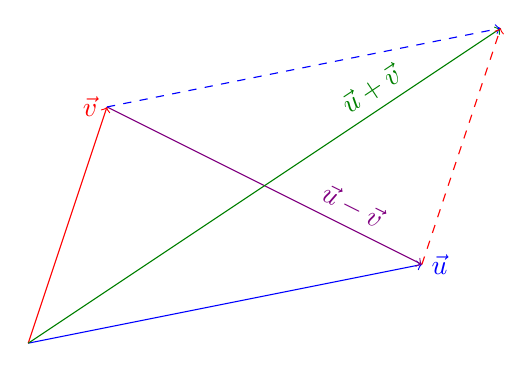
\begin{tikzpicture}
\draw[blue, ->] (0,0) -- (5,1) node[right]{$\vec{u}$};
\draw[red, ->] (0,0) -- (1,3) node[left]{$\vec{v}$};
\draw[Purple, ->] (1,3) -- (5,1) node[pos=0.75, sloped, above]{$\vec{u} - \vec{v}$};
\draw[Green, ->] (0,0) -- (6,4) node[pos=0.75, sloped, above]{$\vec{u} + \vec{v}$};
\draw[blue, dashed, ->] (1,3) -- (6,4);
\draw[red, dashed, ->] (5,1) -- (6,4);
\end{tikzpicture}
\caption{The parallelogram constructed by vectors for Exercise \ref{ex:parallellaw}.}
\label{fig:parallellaw}
\end{figure}
\begin{Answer}
\begin{align*}
\norm{\vec{u}+\vec{v}}^2 + \norm{\vec{u}-\vec{v}}^2 &= (\vec{u}+\vec{v}) \cdot (\vec{u}+\vec{v}) + (\vec{u}-\vec{v}) \cdot (\vec{u}-\vec{v}) \\
&= (\norm{\vec{u}}^2 + 2(\vec{u} \cdot \vec{v}) + \norm{\vec{v}}^2) + (\norm{\vec{u}}^2 - 2(\vec{u} \cdot \vec{v}) + \norm{\vec{v}}^2) \\
&= 2\norm{\vec{u}}^2 + 2\norm{\vec{v}}^2
\end{align*}
\end{Answer}

\begin{Exercise}
Show that Coriolis Force derived in Example \ref{exmp:Coriolis} does zero work and hence is consistent with the fact that it is an apparent force and never produces/consumes energy by itself.
\end{Exercise}
\begin{Answer}
In Example \ref{exmp:Coriolis}, we have
\begin{align*}
\overrightarrow{F_\text{cor}} &= (2\Omega(v\sin\varphi - w\cos\varphi))\hat{i} + (-2\Omega u\sin\varphi)\hat{j} + (2\Omega u\cos\varphi)\hat{k}    
\end{align*}
and hence the rate of work done is
\begin{align*}
&\quad \overrightarrow{F_\text{cor}} \cdot \vec{v} \\
&= [(2\Omega(v\sin\varphi - w\cos\varphi))\hat{i} + (-2\Omega u\sin\varphi)\hat{j} + (2\Omega u\cos\varphi)\hat{k}] \cdot (u\hat{i} + v\hat{j} + w\hat{k}) \\
&= (2\Omega(v\sin\varphi - w\cos\varphi))u + (-2\Omega u\sin\varphi)v + (2\Omega u\cos\varphi)w \\
&= 2\Omega uv\sin\varphi - 2\Omega uw\sin\varphi - 2\Omega uv\sin\varphi + 2\Omega uw\sin\varphi = 0
\end{align*}
Alternatively, note that $\overrightarrow{F_\text{cor}} = -2\overrightarrow{\Omega} \times \vec{v}$ and $({\Omega} \times \vec{v}) \cdot \vec{v} = 0$ always holds.
\end{Answer}